\section{Experimental Evaluation}
\subsection{Experiment Setup}
In all experiments, we set the feature dimension d = 64 and the number of message passing iterations 
T=5 for training. 2GAT + MLP serial connection. The initial number of attention heads is four and is 
increased by one every 1000 steps until eight. We run all experiments on the server using a single 
NVIDIA A100 GPU and eight CPU cores.

We first follow the experiment settings in recent work NSNet. Specifically, we run experiments using the 
same subset of BIRD benchmark\cite{DBLP:conf/aaai/SoosM19} , which contains eight categories arising from DQMR networks, grid 
networks, bit-blasted versions of SMTLIB benchmarks, and ISCAS89 combinatorial circuits. Each category has 
20 to 150 CNF formulas, which we split into training/testing with a ratio of 70\%/30\%. Note that the BIRD 
benchmark is quite small and contains large-sized formulas with more than 10,000 variables and clauses, 
it challenges the generalization ability of our model. Besides evaluating in such a data-limited regime, 
we also conduct experiments on the SATLIB benchmark, an open-source dataset containing a broad range of CNF 
formulas collected from various distributions. To train our model effectively, we choose the distributions 
with at least 100 satisfiable instances, which include the following 5 categories: (1) uniform random 3-SAT 
on phase transition region (RND3SAT), (2) backbone-minimal random 3-SAT (BMS), (3) random 3-SAT with controlled 
backbone size (CBS), (4) "Flat" graph coloring (GCP), and (5) "Morphed" graph coloring (SW-GCP). The whole 
dataset has 46,200 SAT instances with the number of variables ranging from 100 to 600, and we split it into 
training/validation/testing sets with a ratio of 60\%/20\%/20\%. For both BIRD and SATLIB benchmarks, we ran 
the state-of-the-art exact \#SAT solver DSharp\cite{DBLP:conf/ai/MuiseMBH12} with a time limit of 5,000 seconds to generate the 
ground truth labels. The instances where DSharp fails to finish within the time limit are discarded.

\subsection{Evaluation \& Baselines.}
Following BPNN and NSNet, we use the (1) root mean square error (RMSE) between the estimated log countings and 
ground truth as our evaluation metrics. We compare AEIN , the neural baseline BPNN and NSNet, and two state-of-the-art 
approximate model counting solvers, ApproxMC3\cite{DBLP:conf/aaai/SoosM19} and F2\cite{DBLP:conf/sat/AchlioptasHT18a}. For ApproxMC3 and F2, we set a time 
limit of 5,000 seconds on each instance.

\subsection{Main Results}
\begin{figure}[htbp]
    \centering
    \begin{subfigure}{0.48\textwidth}
        \centering
        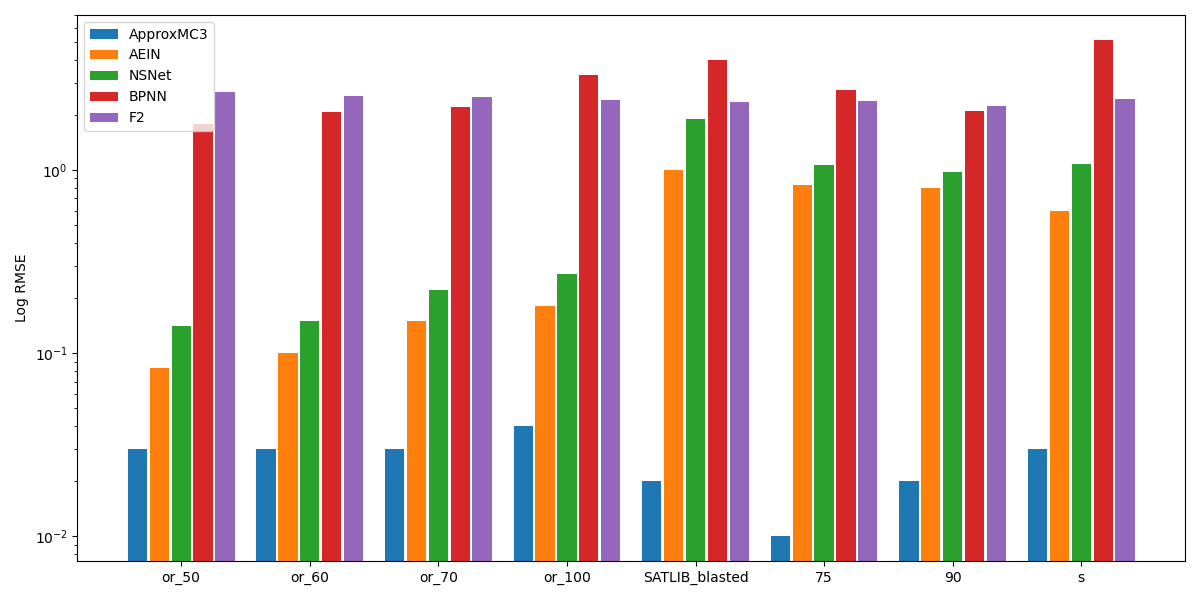
\includegraphics[width=\linewidth]{png/柱状图.png} % 图片1路径
        \caption{}
        \label{fig:sub1}
    \end{subfigure}
    \hfill % 水平填充间距
    \begin{subfigure}{0.48\textwidth}
        \centering
        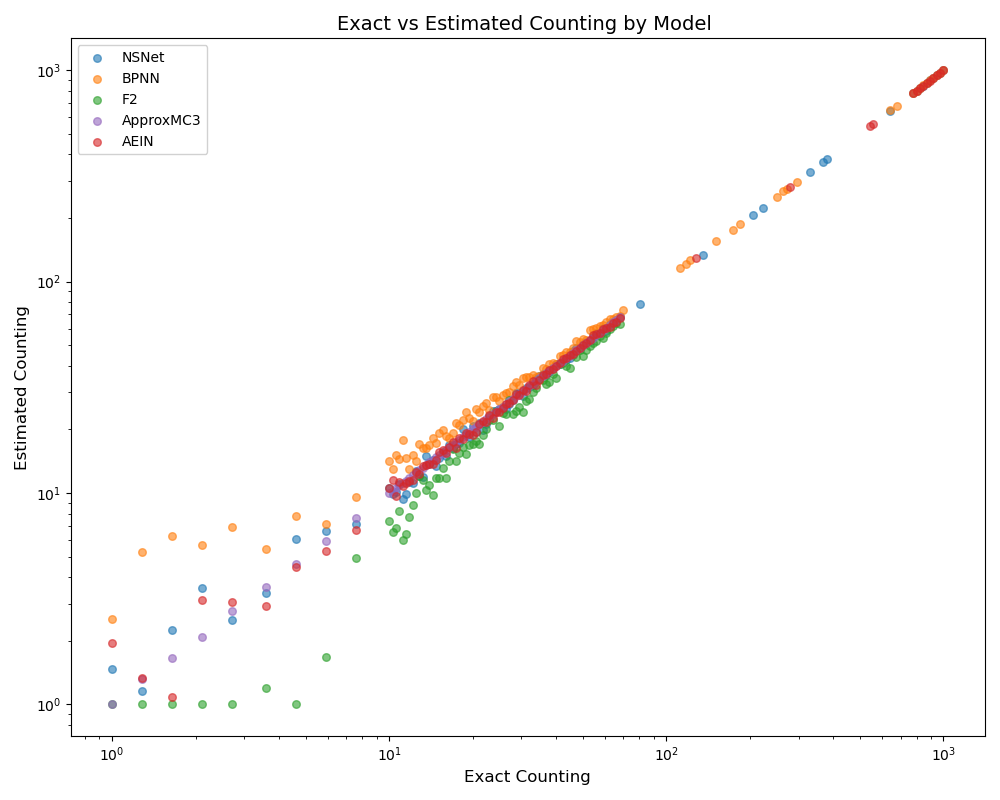
\includegraphics[width=\linewidth]{png/plot.png} % 图片2路径
        \caption{}
        \label{fig:sub2}
    \end{subfigure}
    \caption{(a) is RMSE between estimated log countings and ground truth for each solver on the BIRD benchmark;(b) is Scatter plot comparing the estimated log countings against the ground truth for each solver on the BIRD benchmark}
    \label{fig:total}
\end{figure}

As shown in Figure~\ref{fig:sub1}, AEIN can estimate tighter counts than NSNet, BPNN, and F2 in all categories 
of the BIRD benchmark. AEIN estimates are almost three times more accurate than F2 and BPNN. However, AEIN cannot 
compete with ApproxMC3.

Table 1 shows the detailed RMSE results for each solver on the SATLIB benchmark. All SATLIB datasets were 
generated manually and randomly, and the accuracy decreased compared to the BIRD dataset, but AEIN still 
achieved an advantage in all categories.

Figure~\ref{fig:sub2} shows the scatter plot. The estimated logarithmic count is compared to the ground truth 
for each solver on the BIRD benchmark. When the ground truth is less than \(e^{100}\), AEIN and ApproxMC3 can 
provide more accurate estimates than NSNet, F2 and BPNN in most cases. ApproxMC3 is unable to complete in 5000 
seconds when the ground truth count exceeds \(e^{100}\), AEIN can still give a close approximation when the ground 
truth count exceeds \(e^{1000}\). This demonstrates the effectiveness of AEIN in solving difficult and large cases.

The solution speed of AEIN is of the same order of magnitude as that of NSNet without using the attention mechanism, 
and its effect is still better than that of NSNet. This further indicates that the reasoning ability of the IJGP 
algorithm is superior to that of BP.

\begin{table}[htbp] 
  \centering  
  \caption{Comparison of RMSE between AEIN without attention mechanism and NSNet}  
  \begin{tabular}{ccclll}  
    \toprule
    Method& RND3SAT& BMS & CBS& GCP&SW-GCP\\  
    \midrule
    NSNet& 1.57& 2.45& 1.68& 2.14&1.37\\  
    AEIN-Att& \textbf{1.42}& \textbf{2.29}& \textbf{1.33}& \textbf{2.08}&\textbf{1.25}\\  
    \bottomrule
  \end{tabular}
  \label{tab1}  
\end{table}\\

Table~\ref{tab2} shows the detailed RMSE results for each solver on the SATLIB benchmark. The data for the BIRD benchmark 
is collected from many real-world model counting applications that may share many common logical structures to learn, whereas 
instances in the SATLIB benchmark are randomly generated, making it difficult for AEIN to exploit common features. Despite this, 
AEIN still outperforms NSNet and F2 in most categories.

\begin{table}[htbp] 
  \centering  
  \caption{RMSE between estimated log countings and ground truth for each solver on the SATLIB benchmark.}  
  \begin{tabular}{ccclll}  
    \toprule
    Method& RND3SAT& BMS & CBS& GCP&SW-GCP\\  
    \midrule
    F2& 2.13& 2.42& 2.37& 2.40&2.66\\  
    NSNet& 1.57& 2.45& 1.68& 2.14&1.37\\  
    AEIN& \textbf{1.15}& \textbf{1.66}& \textbf{1.20}& \textbf{1.96}&\textbf{0.96}\\  
    \bottomrule
  \end{tabular}
  \label{tab2}  
\end{table}\\

\begin{table}[htbp] 
  \centering  
  \caption{Ablation experiments of the AEIN model on three refinements.}  
  \begin{tabular}{ccclll}  
    \toprule
    Method& RMSE& Head utilization(\%)& Training time/convergence\\ 
    \midrule
    GAT& 1.33& 100& 185.155\\  
    GAT-H& 1.26& 100& 153.499\\  
    GAT-HC& 1.19& 100& 170.164\\
    \centering  
    GAT-HCD& 1.16& 62.5& 113.165\\  
    \bottomrule
  \end{tabular}
  \label{tab3}  
\end{table}\\

To prove that the three attention mechanisms of our AEIN model are effective, Table~\ref{tab3} shows its ablation experiments with 
RMSE, attention head utilization and training time as evaluation metrics. Experiments show that the three attention mechanisms all 
play a positive role in the model. Among them, the hierarchical attention mechanism and constraint perception mechanism greatly 
improve the accuracy of the model, and the dynamic attention mechanism reduces the redundant attention head over time, avoids more 
calculations, reduces the training time and improves the efficiency of the model.
